\section{Results}
%example network
\FloatBarrier
\begin{figure}[htb!]
    \makebox[\textwidth][c]{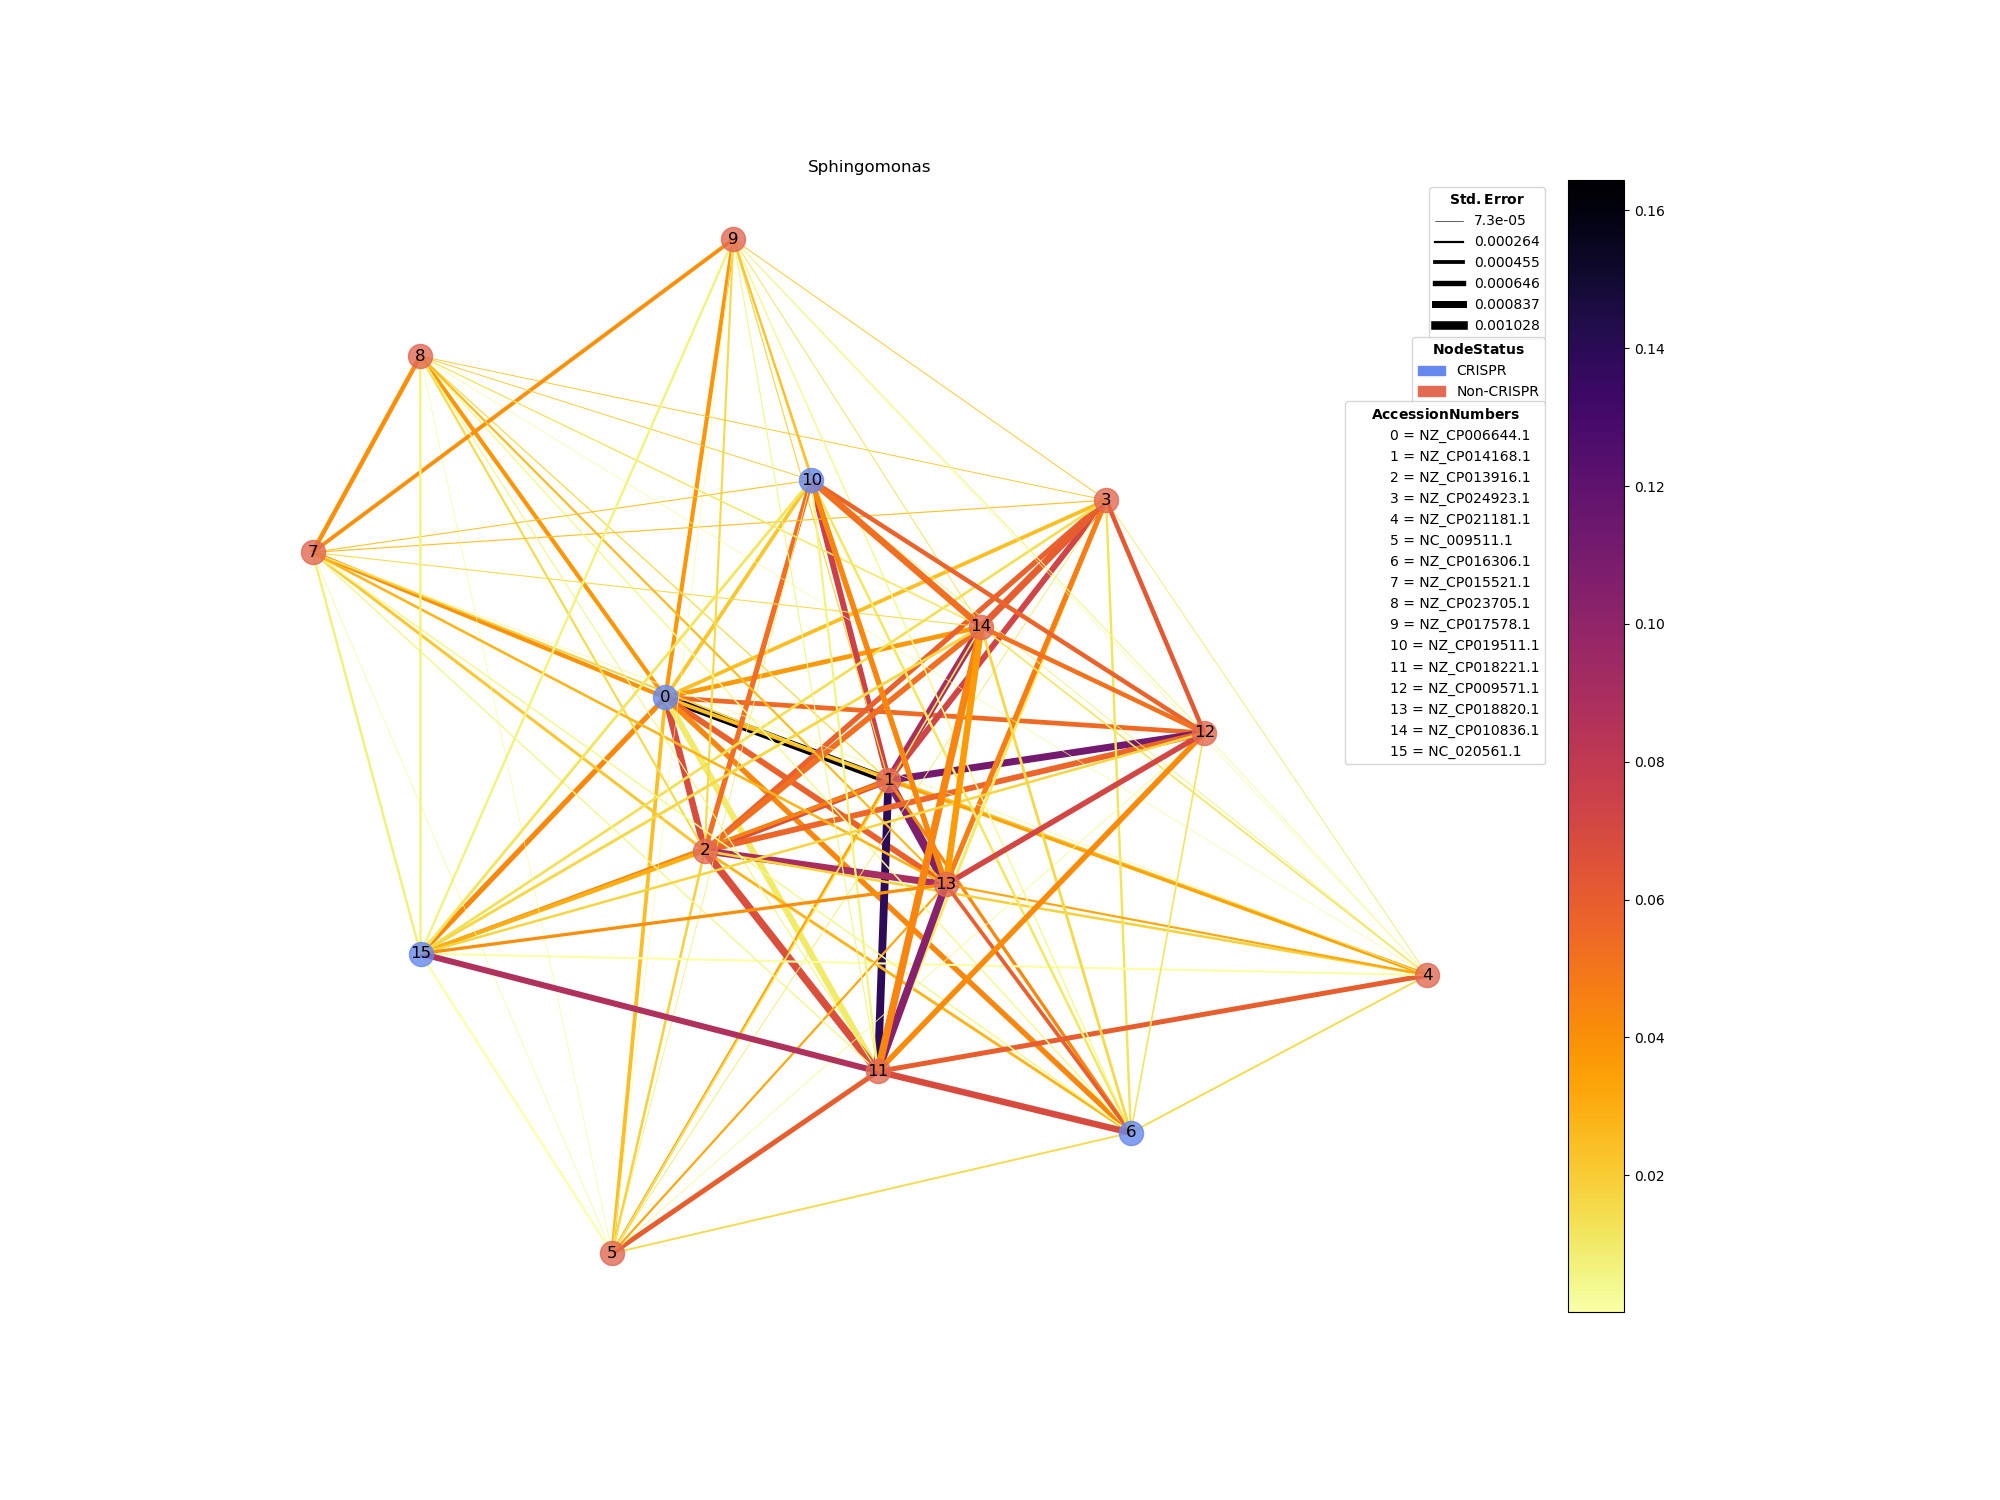
\includegraphics[width=0.8\linewidth]{network.png}}
    \caption{}
    \label{net}
\end{figure}
\FloatBarrier
%degree bar
\FloatBarrier
\begin{figure}[htb!]
    \makebox[\textwidth][c]{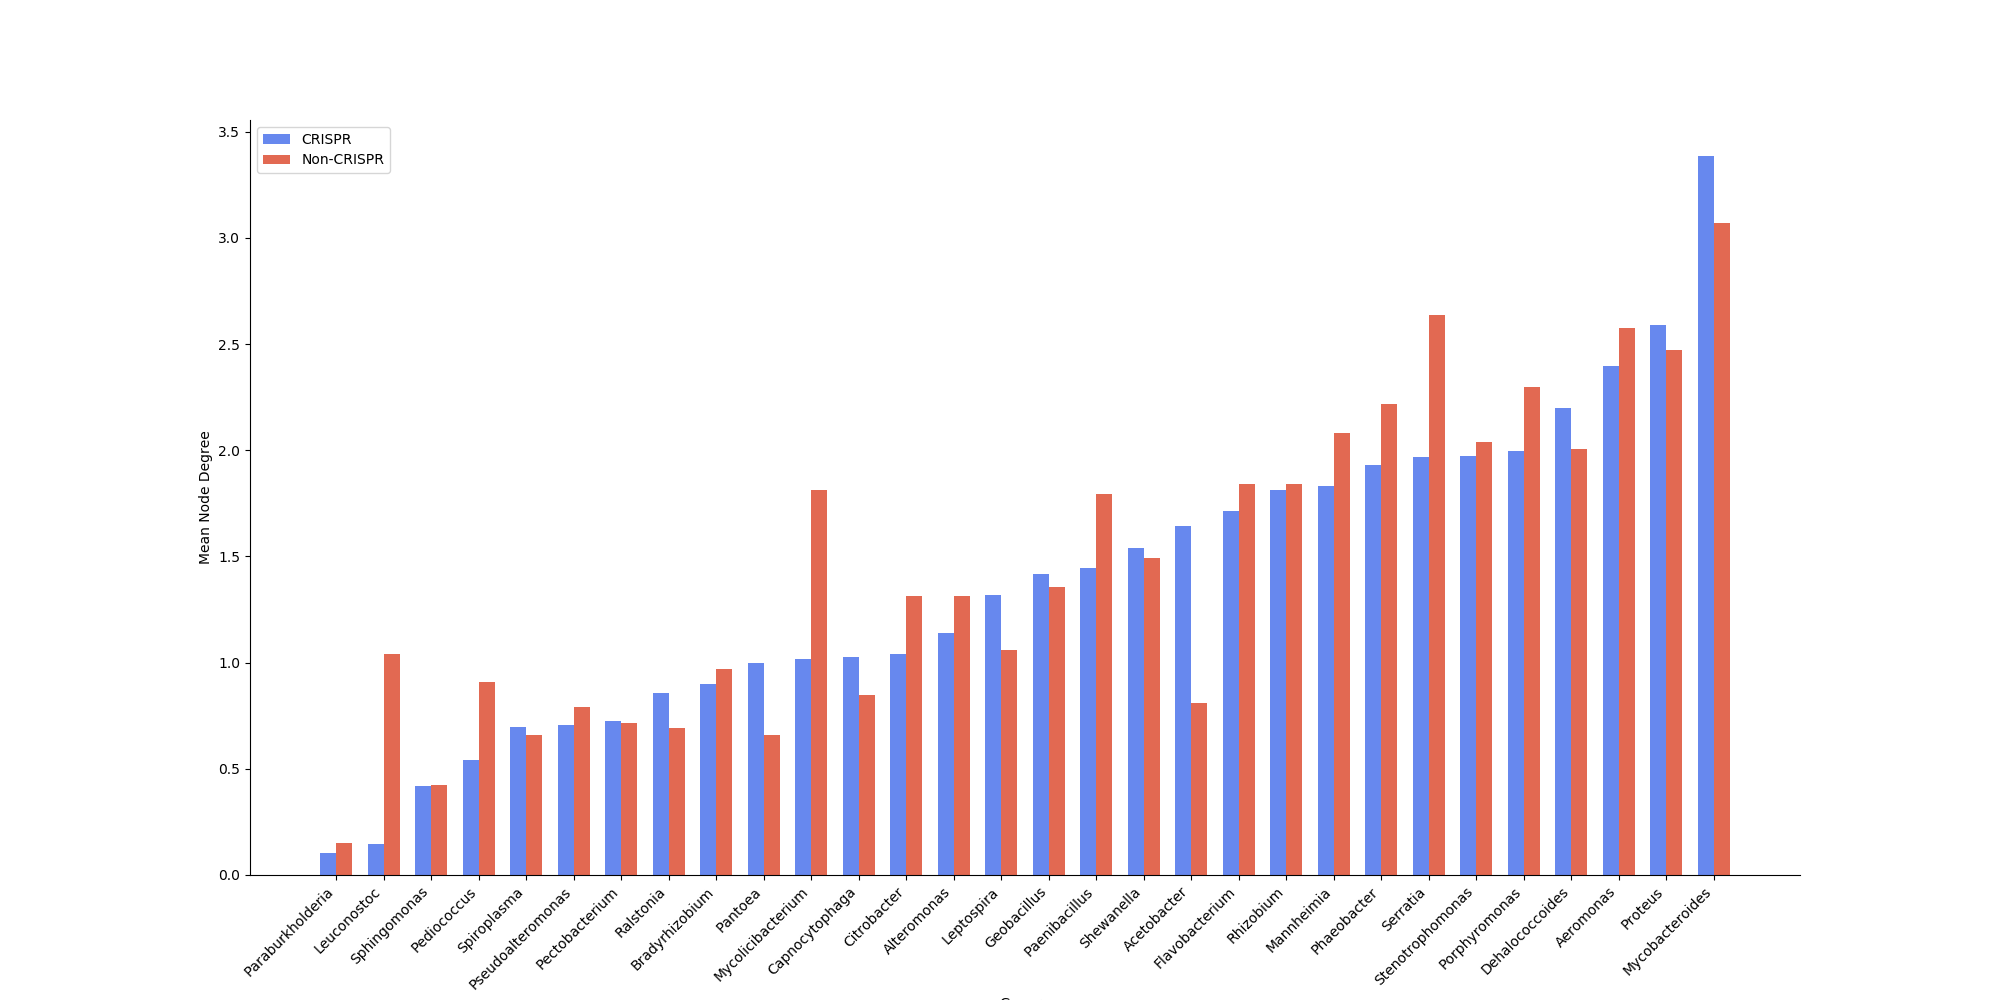
\includegraphics[width=\linewidth]{c_nc_deg_bar.png}}
\end{figure}
\FloatBarrier
%indel bar
\FloatBarrier
\begin{figure}[htb!]
    \makebox[\textwidth][c]{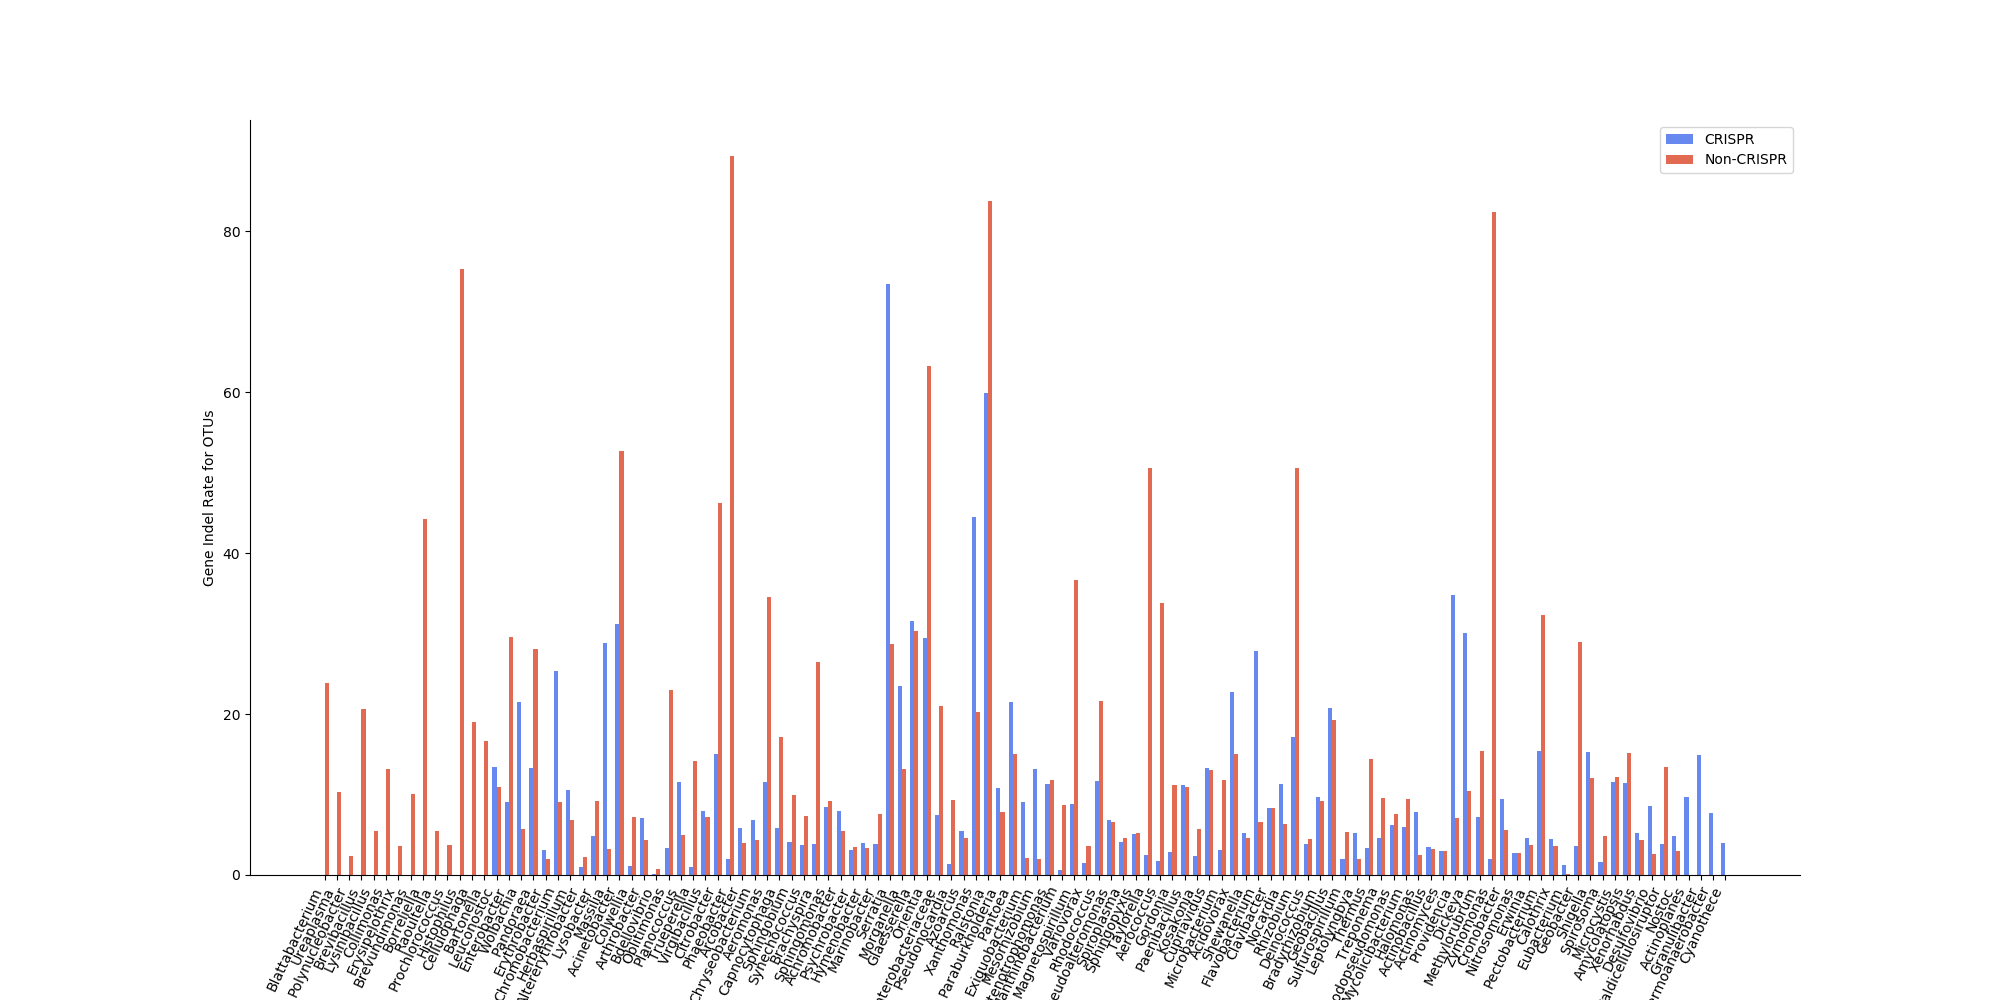
\includegraphics[width=\linewidth]{c_nc_indel_bar.png}}
\end{figure}
\FloatBarrier
%indel scatter
\FloatBarrier
\begin{figure}[htb!]
    \makebox[\textwidth][c]{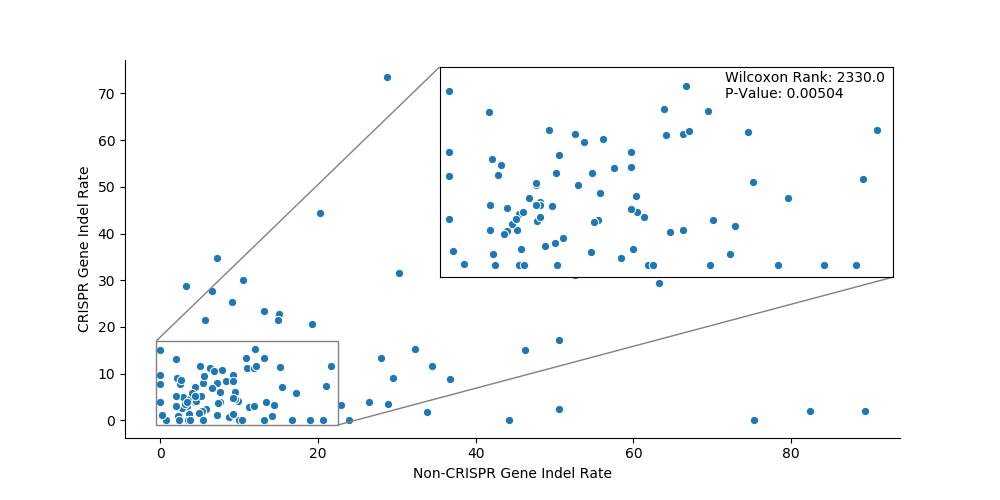
\includegraphics[width=\linewidth]{c_nc_rate_scatter.png}}
\end{figure}
\FloatBarrier
%Cfrac vs rate difference
\FloatBarrier
\begin{figure}[htb!]
    \makebox[\textwidth][c]{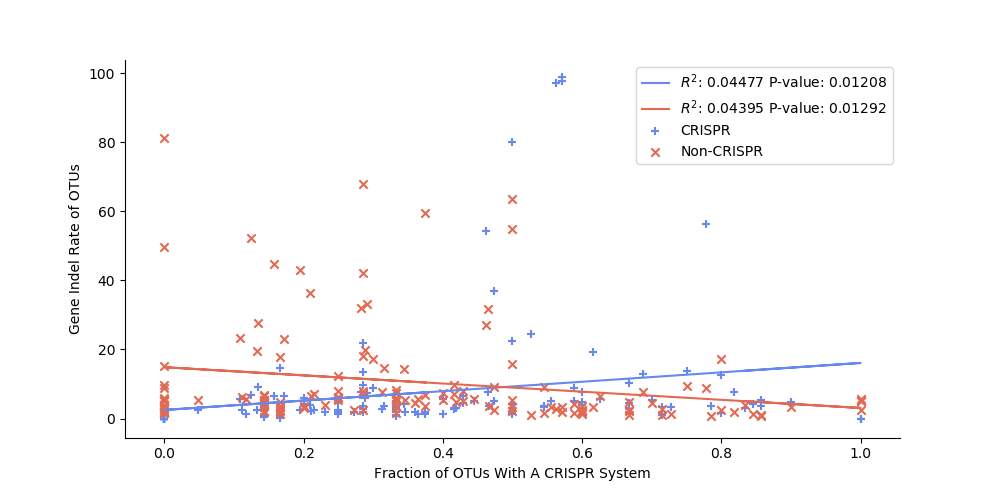
\includegraphics[width=\linewidth]{cfrac_cncRateDiff_scattter.png}}
\end{figure}
\FloatBarrier
%Cluster C NC
\FloatBarrier
\begin{figure}[htb!]
    \makebox[\textwidth][c]{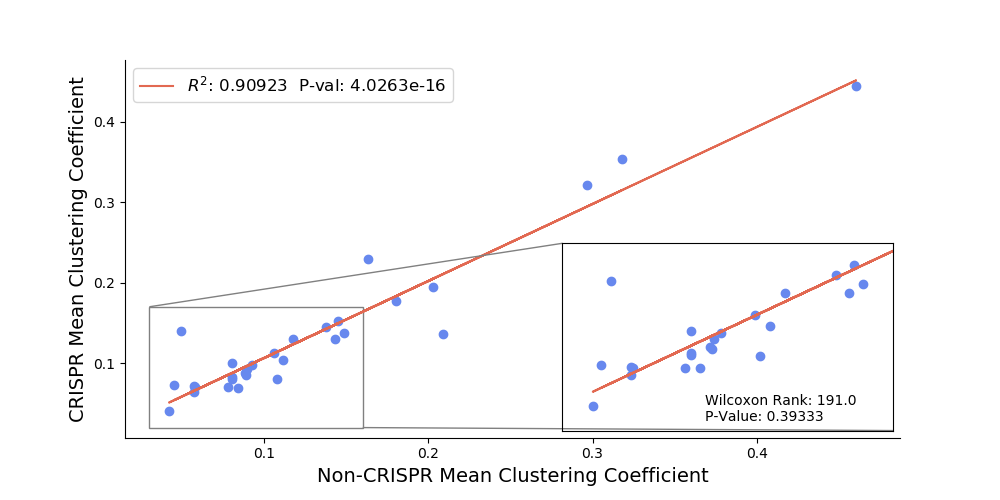
\includegraphics[width=\linewidth]{c_nc_clust_scatter.png}}
\end{figure}
\FloatBarrier
%modularity
\FloatBarrier
\begin{figure}[htb!]
    \makebox[\textwidth][c]{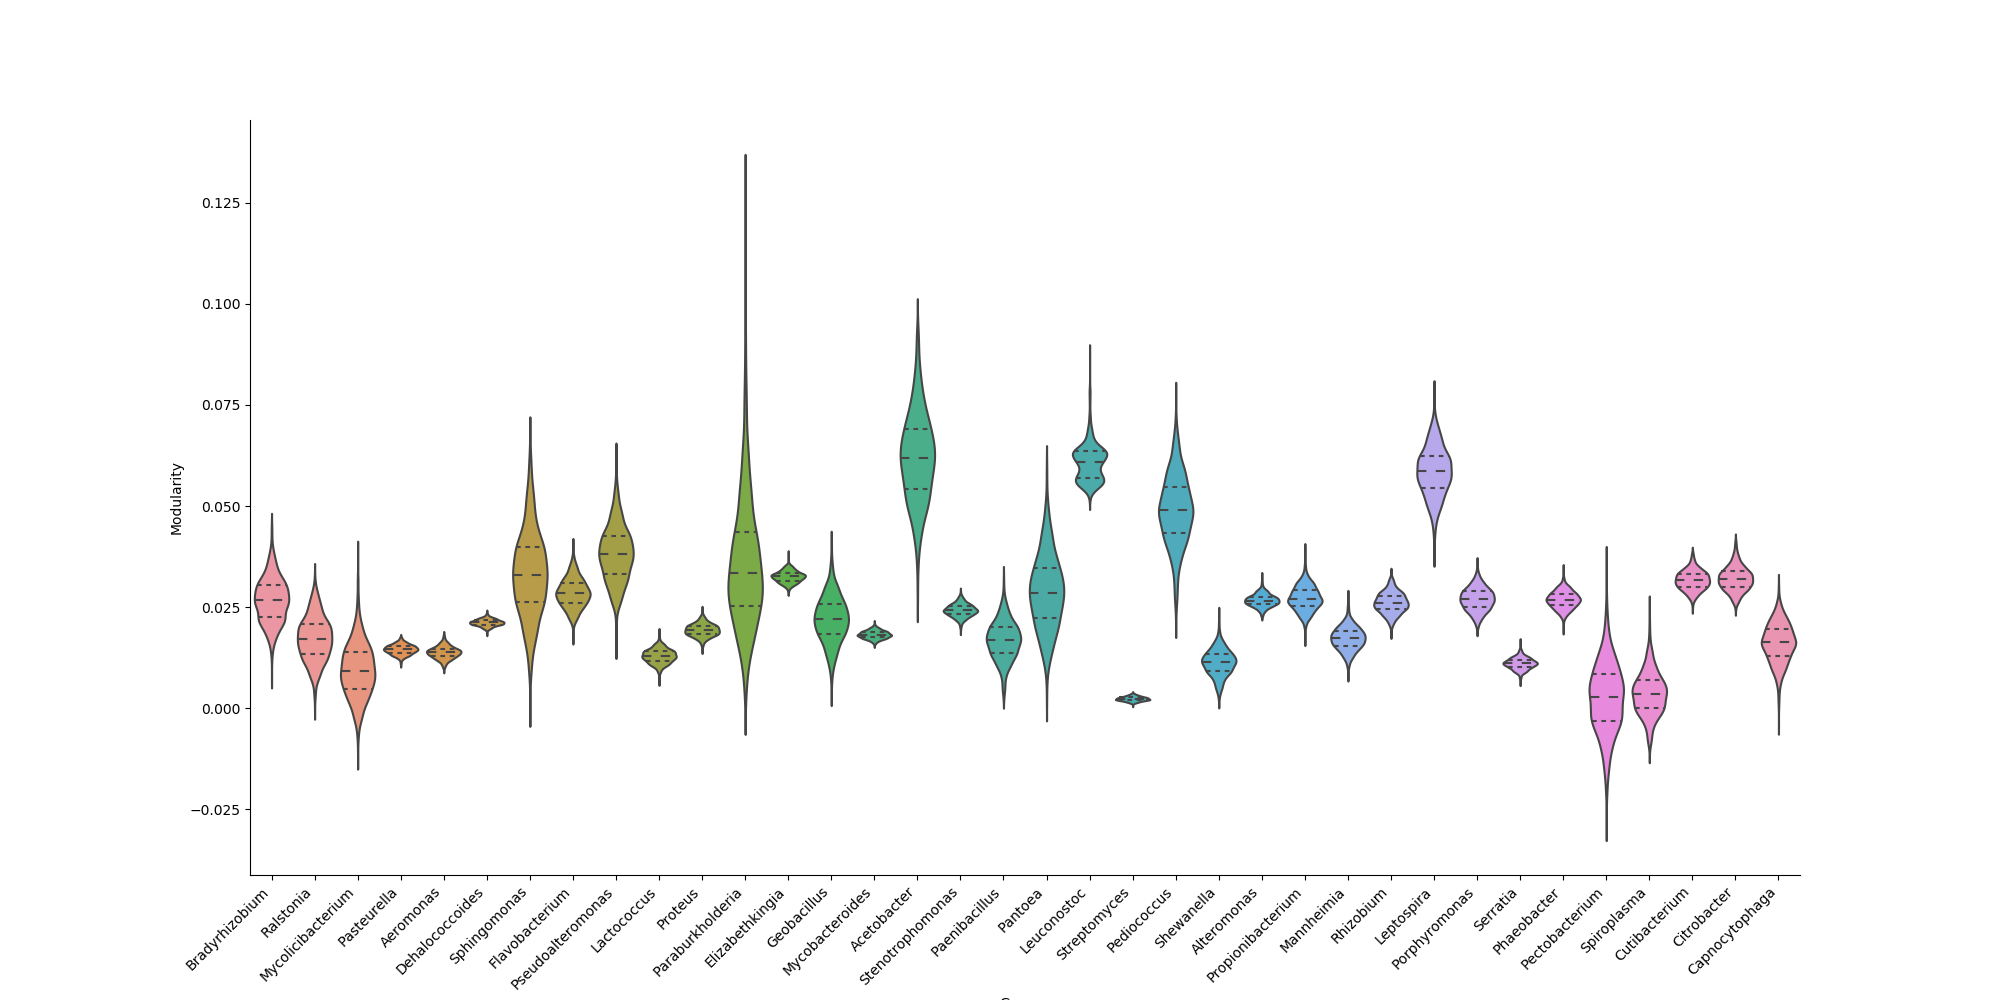
\includegraphics[width=\linewidth]{mod_violin.png}}
\end{figure}
\FloatBarrier
%Assortativity
\FloatBarrier
\begin{figure}[htb!]
    \makebox[\textwidth][c]{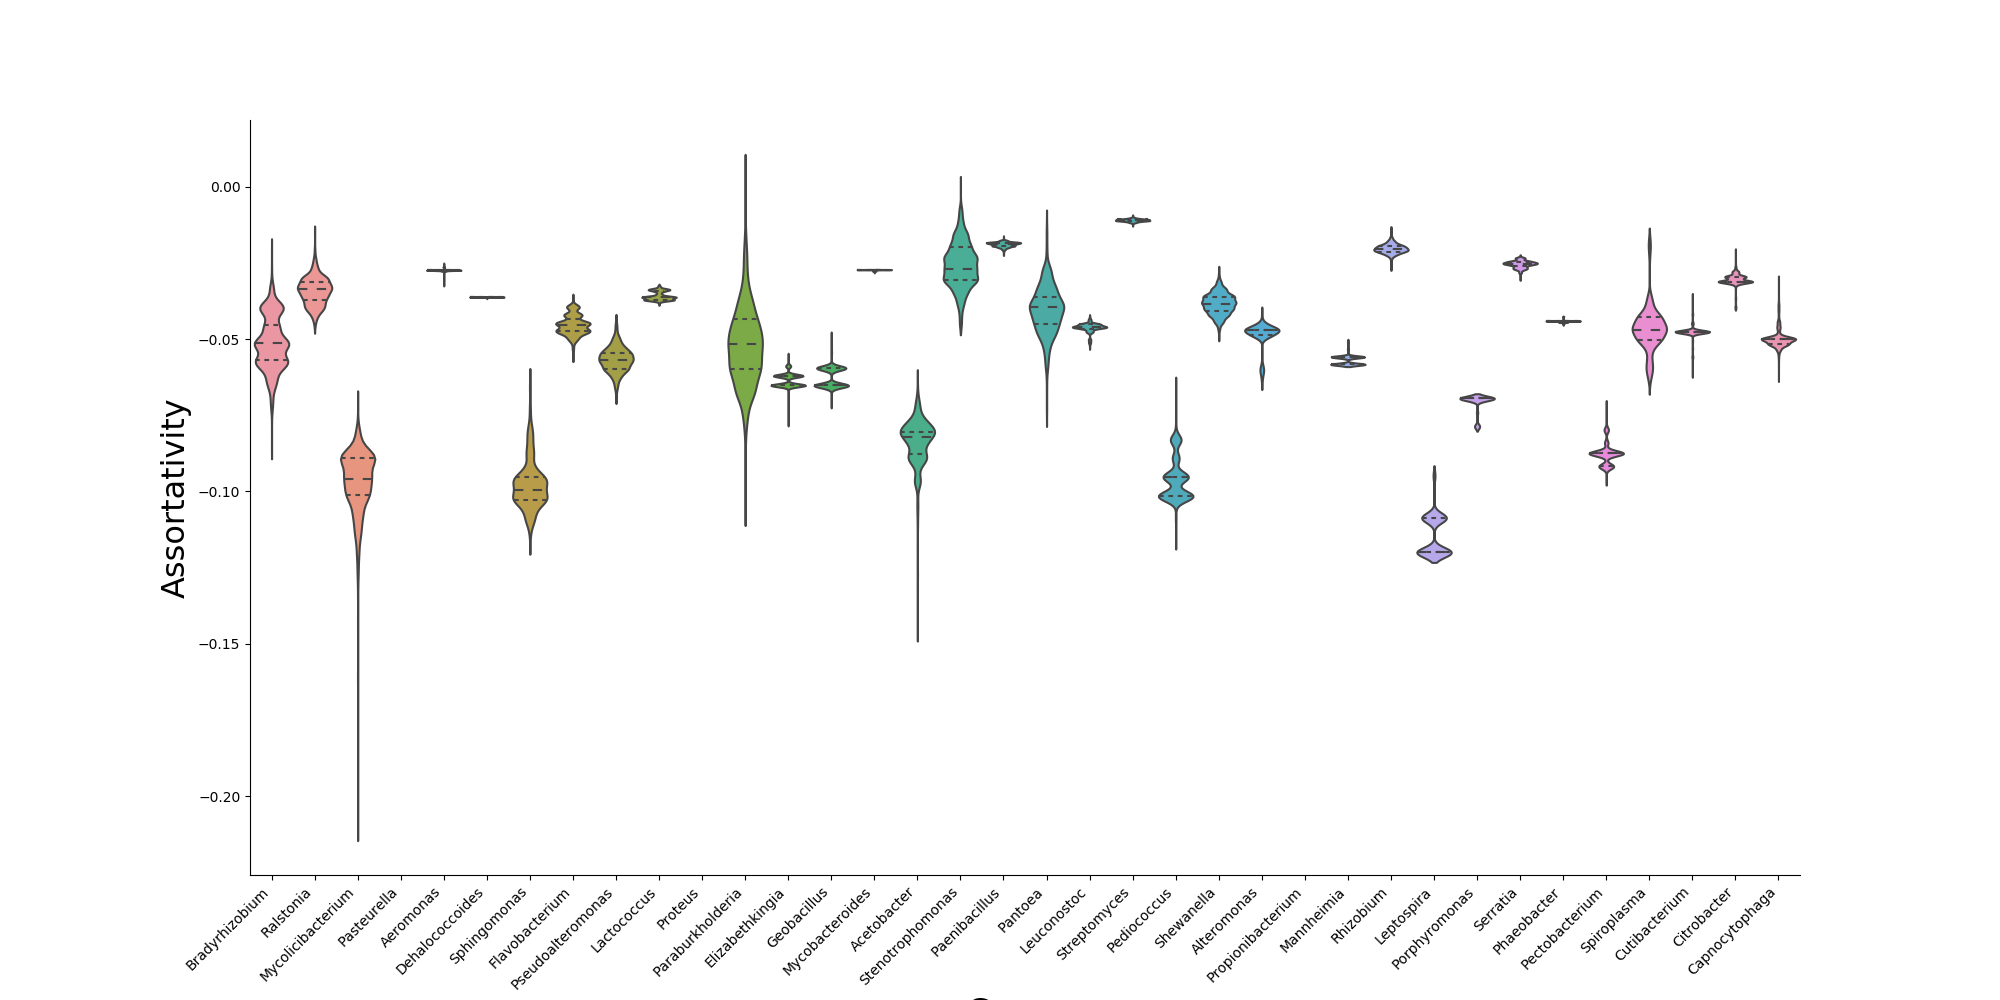
\includegraphics[width=\linewidth]{asst_violin.png}}
\end{figure}
\FloatBarrier
%pairplot
\FloatBarrier
\begin{figure}[htb!]
    \makebox[\textwidth][c]{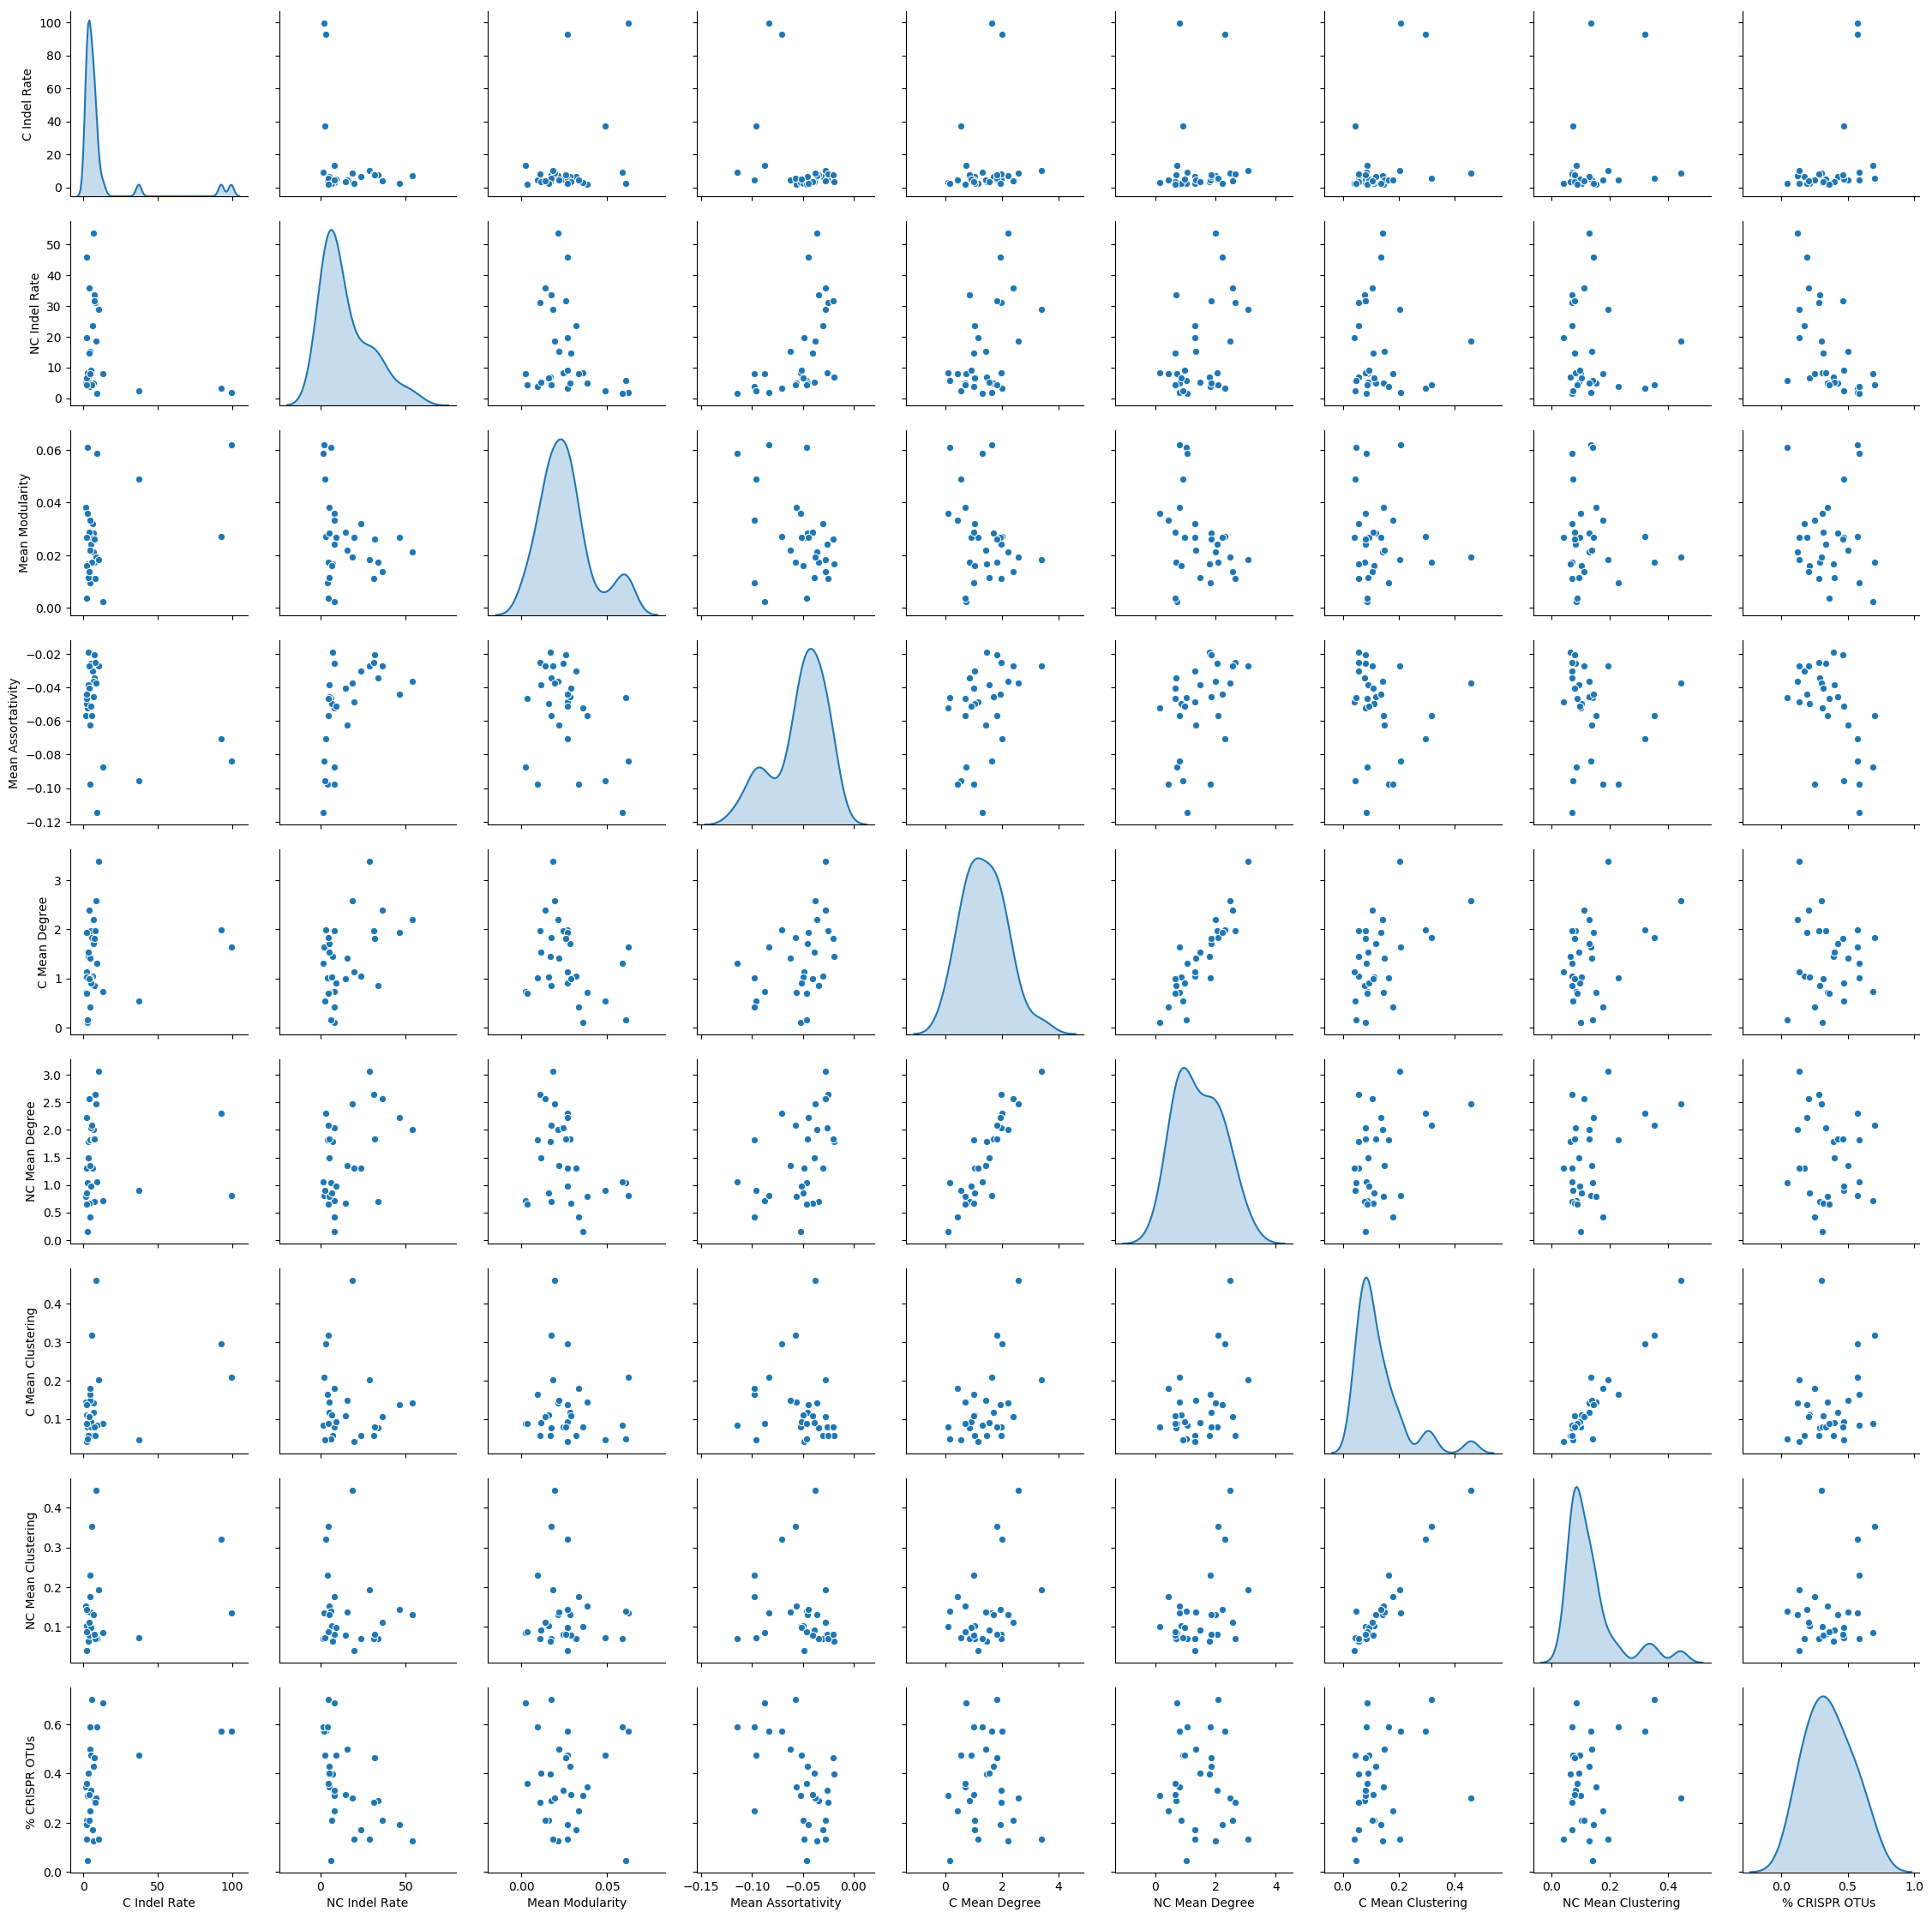
\includegraphics[width=\linewidth]{pairplot.png}}
\end{figure}
\FloatBarrier
